\chapter{Conclusions}
\label{con}
\section{Summary of Results}
The HELIOS spectrometer was successfully commissioned using the ($d$,$p$) neu\-tron-\-trans\-fer reaction
on $^{28}$Si in inverse kinematics at 6.0 MeV/$u$.
The purpose of the commissioning experiment was to verify the resolution, acceptance, and transport properties suggested by the design of this novel spectrometer.   Analytical calculations and Monte Carlo simulations were carried out to model the performance of the spectrometer and the experimental results were in excellent agreement, as demonstrated in Figs.~\ref{hEZ} and \ref{b11_spec}.  This experiment demonstrated that a $Q$-value resolution of less than 80\,keV~FWHM in inverse kinematics is attainable with HELIOS.  This remarkable result approaches those of measurements made in normal kinematics.  

The large acceptance of HELIOS was established with this measurement covering nearly $50^\circ$ in the center-of-mass frame ($\Delta \Omega=1.18$\,sr), and proton energies from 210\,keV to over 9\,MeV.  The performance properties unique to solenoidal transport provided by HELIOS were also confirmed.  Namely, the time-of-flight of the detected ions was approximately the cyclotron period $T_\mathrm{cyc}$, providing $A/q$ particle identification and the measured kinematic groups were separated by their excitation energy $\Delta E_\mathrm{lab}=\Delta E_\mathrm{cm}$.  %  The commissioning experiment was an overall success.

The enhanced resolution of the HELIOS spectrometer is due to the linear correlation between the measured quantities $z$ and $E_\mathrm{lab}$.  This relationship eliminates kinematic compression and dramatically suppresses resolution broadening due to the kinematic covariation of the measured quantities.  Comparing excitation energy spectra produced with HELIOS (Figs.~\ref{qval} and \ref{b11b12_spec_helios}) to state-of-the-art measurements made in conventional detector geometry (Figs.~\ref{b11b12_spec} and \ref{133Sn_e}), it is clear that HELIOS has substantially superior center-of-mass energy resolution ($\approx3\times$).  Based on the advantages of the HELIOS spectrometer, it is clear that HELIOS is the ideal instrument for measuring the $d$($^{132}$Sn,$p$)$^{133}$Sn reaction.  Its unique geometry provides the high-efficiency, high-resolution measurements required by inverse kinematics.  

\section{Outlook}
\subsection[\texorpdfstring{The $^\text{132}$S\lowercase{n($d$,$p$)} Measurement}{The 132Sn(d,p) Measurement}]{\texorpdfstring{The $^\mathbf{132}$Sn($d$,$p$) Measurement}{The 132Sn(d,p) Measurement}}
The future of HELIOS measurements utilizing rare isotope beams far from stability is dependent on the full completion of the Californium Rare Isotope Beam Upgrade (CARIBU) radioactive ion source, currently  undergoing the final stages of development.
As of this writing, the $^{132}$Sn($d$,$p$) reaction has not yet been measured with HELIOS.  However, the opportunity to carry out this measurement is on the near horizon. 
 In March, 2011, the CARIBU ion source was successfully commissioned.  A beam of $^{143}$Ba ions ($T_{1/2}=14.5$\,s) produced by CARIBU was detected at the ATLAS High-Energy Diagnostics region, % at an intensity of 625\,pps.  The beam had an energy of 6.1\,AMeV as was
  identified by the characteristic $\gamma$-decay spectrum.  While a $^{132}$Sn beam has not yet been produced, HELIOS has been used to measure an $N=82$ heavy ion reaction, specifically ($d$,$p$) on $^{136}_{~54}$Xe~\cite{Kay_2011}.  

Fig.~\ref{fig2} shows the characteristic $E$ vs. $z$ spectrum $d$($^{136}$Xe,$p$)$^{137}$Xe reaction at 10\,\AMeV and $\mathscr{B}_0=2$\,T for two target-array positions.  These data are gated on events corresponding to a cyclotron period of 32.8\,ns---the cyclotron period for protons at 2\,T. The background is protons from fusion-evaporation of target and beam.  Fig.\ref{fig2} also shows the excitation energy spectrum measured in this experiment; 11 states above $E_x=1.5$\,MeV had quantities identified or derived for the first time in this measurement.  The $Q$-value resolution of this measurement is $\Delta E_\mathrm{cm}=100$\,keV~FWHM, which is consistent with the lighter mass studies discussed in Chapt.~\ref{exp}. 
In addition, angular distributions were measured for several states.  This measurement demonstrates that the HELIOS spectrometer is poised for an effective and groundbreaking measurement of the $^{132}$Sn($d$,$p$) reaction.  Part of a successful measurement of $^{132}$Sn($d$,$p$) with HELIOS would possibly involve the first-ever measurement of angular distributions of states in $^{133}$Sn above $E_x=1$\,MeV

\subsection{Instrumental Improvements}
\label{instr}
While the results of the commissioning experiment are very encouraging, the present implementation
of HELIOS is still that of a demonstration prototype.  A number of
improvements to the apparatus are planned, including new silicon
detectors in an arrangement that will provide twice the solid-angle
coverage and improved overall resolution, as well as greater
center-of-mass-angle acceptance.  The new array will be hexagonal in cross section, modular in 5-detector lengths.  Also planned is the addition of a
gas parallel-plate avalanche counter and ionization chamber for the
detection and identification of recoiling heavy nuclei that cannot be
so identified using silicon $\Delta E-E$ techniques.  While the
present spectrometer configuration is tailored to the detection of
particles emitted with laboratory angles greater than $\theta_\mathrm{lab}=90^\circ$, the
advantages of simplified kinematics and improved resolution also apply
to reactions in inverse kinematics that emit light ions
forward of $\theta_\mathrm{lab}=90^\circ$, such as $(d,^3$He).  As of this writing, the silicon detector array has been moved to the downstream position and additional work is currently underway
to accommodate such $K>1$ reactions.    With these features in mind, it is clear that HELIOS is a powerful tool for measuring nuclear reactions in inverse kinematics.

\begin{figure*}[h!]
\centering
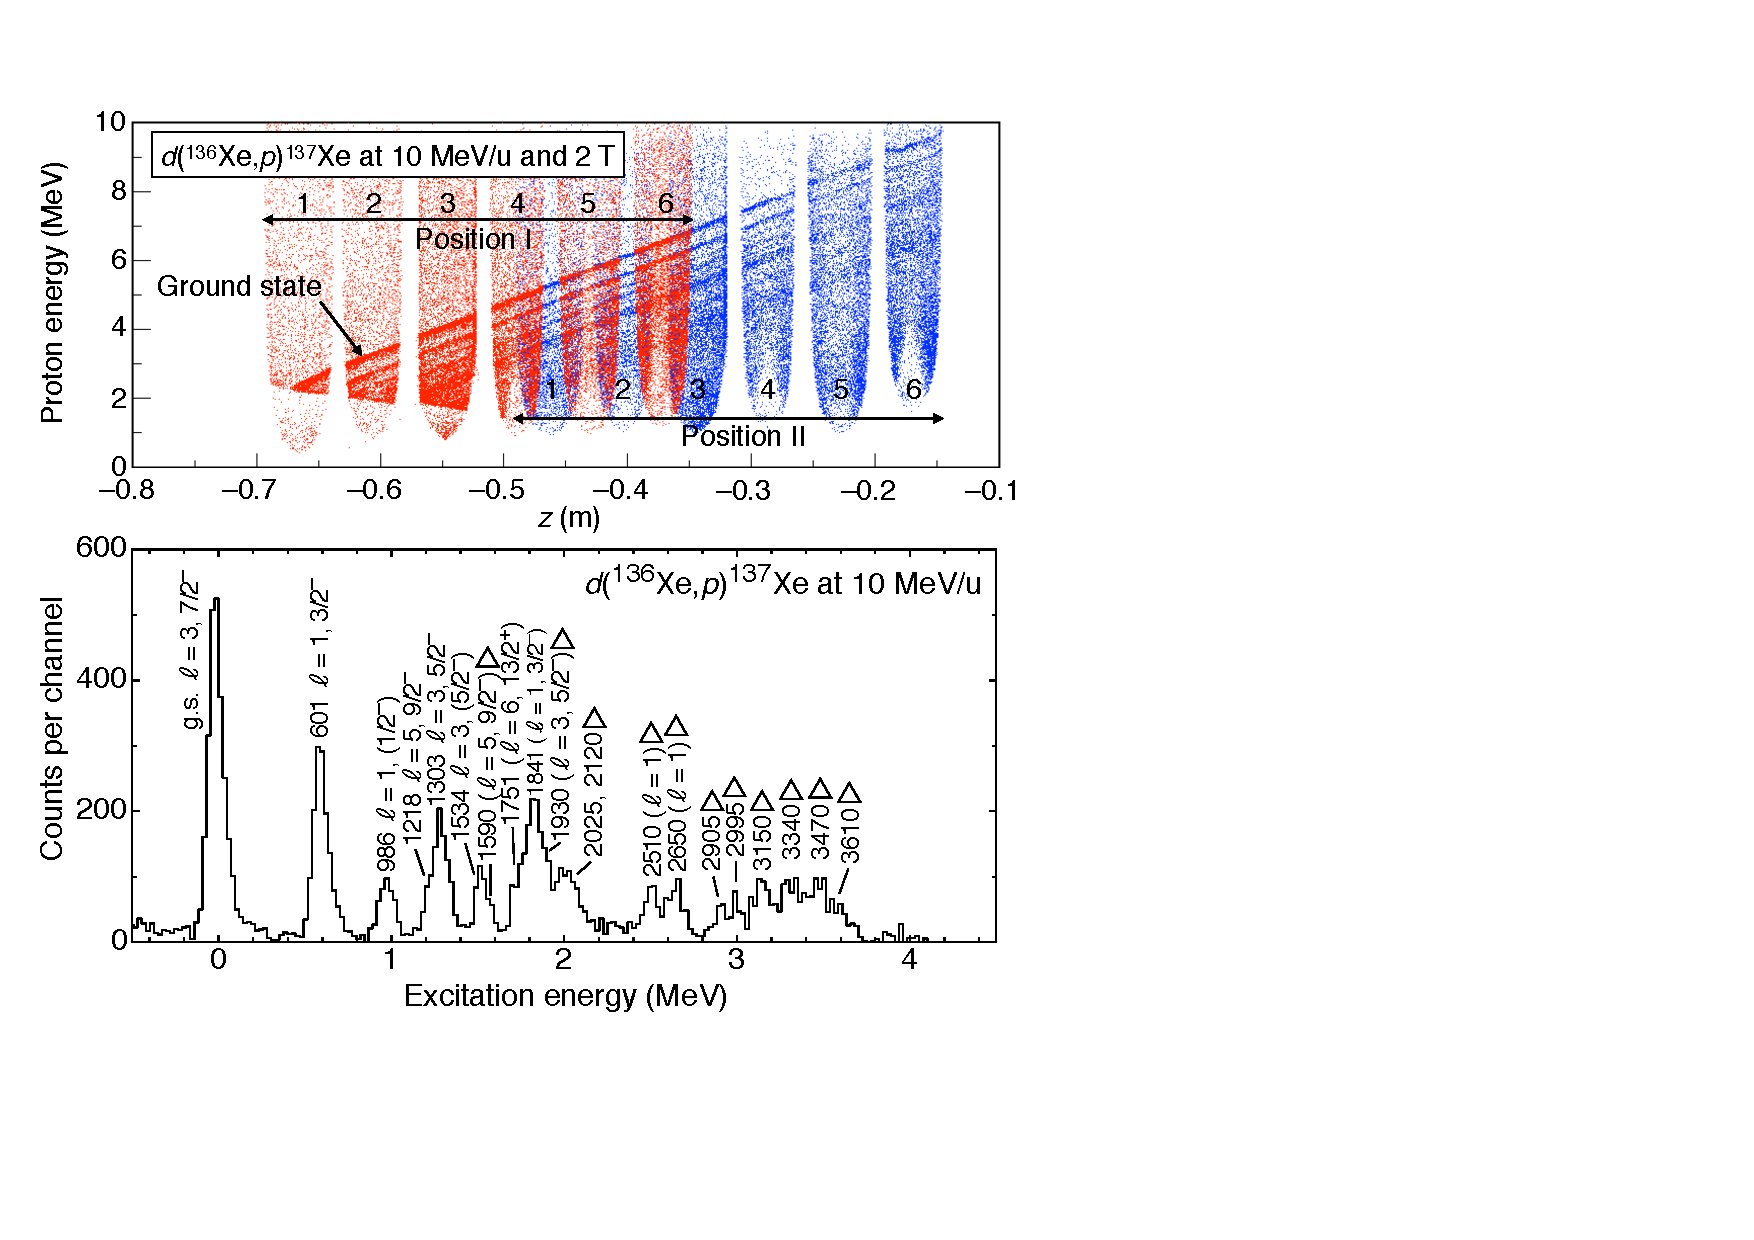
\includegraphics[width=\columnwidth,height=0.9\textheight,keepaspectratio]{fig2}%
\caption[$E$ vs. $z$ and excitation energy spectrum for the $d$($^{136}$Xe,$p$)$^{137}$Xe reaction]{(color online) (Top) Energy vs. position spectrum for the $d$($^{136}$Xe,$p$)$^{137}$Xe reaction at 10\,\AMeV and $\mathscr{B}_0=2$\,T for two target-array positions; $\Delta z=50$\,mm (blue) and $\Delta z=350$\,mm (red), as indicated by the horizontal lines. 
(Bottom) Excitation energy spectrum for $^{137}$Xe.  Peaks are labeled with their energy, and where known, their $\ell$-value, spin, and parity. States marked with a $\triangle$ symbol are those with energy, $\ell$-value, or both, deduced for the first time in this work. Spins and parities in parentheses are to be regarded as tentative. A smooth background (evaporated protons from $^{136}\textrm{Xe} + ^{12}$C fusion) has been subtracted. Figures by B.~P.\ Kay~\cite{Kay_2011}.}
\label{fig2} 
\end{figure*}